\documentclass[12pt]{scrreprt}
\usepackage[utf8]{inputenc}
\usepackage{blindtext, xcolor}
\usepackage{comment}
\usepackage{enumerate}
\usepackage{booktabs}
\usepackage{multirow}
\usepackage[shortlabels]{enumitem}
\usepackage{graphicx}
\usepackage{tabularx}
\renewcommand\tabularxcolumn[1]{m{#1}}
\usepackage{mathtools}
\usepackage{mathpazo}
\usepackage{mdframed} 
\usepackage{float}
\usepackage{mdwlist}
\usepackage{alphabeta}
\usepackage{makecell}
\usepackage{pdflscape}
\usepackage{geometry}
\usepackage{colortbl}
%---------------------------------------------------------------------------
%--------------------------------------------------------------------------- 
% Full justification with typewriter font 
%--------------------------------------------------------------------------- 
\usepackage{everysel} 
\EverySelectfont{% 
\fontdimen2\font=0.4em% interword space 
\fontdimen3\font=0.2em% interword stretch 
\fontdimen4\font=0.1em% interword shrink 
\fontdimen7\font=0.1em% extra space 
\hyphenchar\font=`\-% to allow hyphenation 
} 
\usepackage[pagewise]{lineno}
%\usepackage[htt]{hyphenat} % Trennung von Typewriter Fonts
\def\linenumberfont{\normalfont\small}
\usepackage{svg}
%\usepackage{glossaries}
\usepackage[acronym,numberedsection]{glossaries}
\usepackage[nohyperlinks, printonlyused, withpage]{acronym}
\usepackage{listings}
\usepackage{color}
% deutsche Silbentrennung
%\usepackage[ngerman]{babel}
\usepackage[english]{babel}
% fuer Stichwortverzeichnis 
\usepackage{makeidx}
\usepackage{marvosym}
\usepackage{scrlayer-scrpage}
%\usepackage[headsepline,footsepline,plainfootsepline,markcase=upper]{scrlayer-scrpage}
\usepackage{url}
\usepackage{setspace}
\usepackage{csquotes}

%---------------------------------------------------------------------------
%---------------------------------------------------------------------------
% custom packages go here
\usepackage{xfrac}
%\usepackage{array}
%\usepackage{ragged2e}
\usepackage{boldline} 
\usepackage{array}
\newcolumntype{?}{!{\vrule width 2pt}}
\usepackage{tocloft}
\newcommand{\listequationsname}{}
\newlistof{myequations}{equ}{\listequationsname}
\newcommand{\myequations}[1]{%
\addcontentsline{equ}{myequations}{\protect\numberline{\theequation}#1}\par}
\newcommand\tab[1][3.5cm]{\hspace*{#1}}
%--------------------------------------------------------------------------- 

\usepackage{everysel}
\onehalfspacing
%adi
\setlength{\headheight}{1.1\baselineskip}
%\usepackage[style=apa, backend=biber, language=ngerman]{biblatex}
\usepackage[style=apa, backend=biber, language=english]{biblatex}
%\DeclareLanguageMapping{ngerman}{ngerman-apa} 
\DeclareLanguageMapping{american}{american-apa}
\addbibresource{References.bib} 

\bibliography{References}
\renewcommand*{\chapterheadstartvskip}{\vspace*{0cm}}
% http://tex.stackexchange.com/questions/19738/why-doesnt-pagestyleempty-work-on-the-first-page-of-a-chapter
\renewcommand*\chapterpagestyle{scrheadings}
 
%\restylefloat{table}

\definecolor{dkgreen}{rgb}{0,0.6,0}
\definecolor{mauve}{rgb}{0.58,0,0.82}
\definecolor{gray}{rgb}{0.4,0.4,0.4}
\definecolor{darkblue}{rgb}{0.0,0.0,0.6}
\definecolor{cyan}{rgb}{0.0,0.6,0.6}

\lstset{frame=tb,
	captionpos=b,
	language=Java,
	aboveskip=3mm,
	belowskip=3mm,
	showstringspaces=false,
	columns=flexible,
	basicstyle={\small\ttfamily},
	numbers=none,
	numberstyle=\tiny\color{gray},
	keywordstyle=\color{blue},
	commentstyle=\color{dkgreen},
	stringstyle=\color{mauve},
	breaklines=true,
	breakatwhitespace=true,
	tabsize=3
}

\lstdefinelanguage{XML}
{
	morestring=[b]",
	morestring=[s]{>}{<},
	morecomment=[s]{<?}{?>},
	stringstyle=\color{black},
	identifierstyle=\color{darkblue},
	keywordstyle=\color{cyan},
	morekeywords={xmlns,version,type}% list your attributes here
}

\usepackage{datetime2}
\newcommand\docversion{DRAFT \today\hspace{0.1cm}\DTMcurrenttime}


\usepackage{listingsutf8}

\lstdefinelanguage{docker}{
  keywords={FROM, RUN, COPY, ADD, ENTRYPOINT, CMD,  ENV, ARG, WORKDIR, EXPOSE, LABEL, USER, VOLUME, STOPSIGNAL, ONBUILD, MAINTAINER},
  keywordstyle=\color{blue}\bfseries,
  identifierstyle=\color{black},
  sensitive=false,
  comment=[l]{\#},
  commentstyle=\color{purple}\ttfamily,
  stringstyle=\color{red}\ttfamily,
  morestring=[b]',
  morestring=[b]"
}

\lstdefinelanguage{docker-compose}{
  keywords={image, environment, ports, container_name, ports, volumes, links},
  keywordstyle=\color{blue}\bfseries,
  identifierstyle=\color{black},
  sensitive=false,
  comment=[l]{\#},
  commentstyle=\color{purple}\ttfamily,
  stringstyle=\color{red}\ttfamily,
  morestring=[b]',
  morestring=[b]"
}
\lstdefinelanguage{docker-compose-2}{
  keywords={version, volumes, services},
  keywordstyle=\color{blue}\bfseries,
  keywords=[2]{image, environment, ports, container_name, ports, links, build},
  keywordstyle=[2]\color{olive}\bfseries,
  identifierstyle=\color{black},
  sensitive=false,
  comment=[l]{\#},
  commentstyle=\color{purple}\ttfamily,
  stringstyle=\color{red}\ttfamily,
  morestring=[b]',
  morestring=[b]"
}

\lstset{basicstyle=\ttfamily,
  showstringspaces=false,
  commentstyle=\color{red},
  keywordstyle=\color{blue},
  inputencoding=utf8,
  extendedchars=true
}


% Umbenennung einer Einträge
%\renewcommand\tablename{Tabelle}
%\renewcommand{\figurename}{Abbildung}
%With babel (and English as language):
%\addto\captionsenglish{\renewcommand{\figurename}{Fig.}}
%\renewcommand\bibname{\section{Literaturverzeichnis}}
\renewcommand\bibname{\section{Bibliography}}
%\renewcommand*\contentsname{Inhaltsverzeichnis}
%\renewcommand{\glossaryname}{Sachwortverzeichnis}
%\renewcommand{\indexname}{\section{Sachwortverzeichnis}}
%\renewcommand{\acronymname}{\section{Abkürzungsverzeichnis}}
%\renewcommand{\listfigurename}{\section{Abbildungsverzeichnis}}
%\renewcommand{\listtablename}{\section{Tabellenverzeichnis}}
%\renewcommand\lstlistingname{Listing}
%\renewcommand\lstlistlistingname{\section{Listingverzeichnis}}

% disable indention of paragraphs
\setlength{\parindent}{0pt}

% Damit auch subsubsections nummeriert werden und im ToC auftauchen
\setcounter{secnumdepth}{3}
\setcounter{tocdepth}{2}

\makeindex
\pagestyle{scrheadings}
\clearscrheadfoot
\ihead{
\includegraphics[height=1.69cm]{images/FH-burgenland-logo_white.png}}
\ohead{
	\\ \vspace{15px} \textnormal{\footnotesize{Department Informationtechnology}}
	%\par\nobreak\vspace{-8px}\makebox{\rule{\textwidth}{0.4pt}}
	\par\nobreak\vspace{-12px}\line(30,0){325}
	}
\ofoot{
	\pagemark
	\par\nobreak\vspace{-12px}\makebox[\linewidth]{\rule{\textwidth}{0.4pt}}
	\\
	\textnormal{%Bachelorstudiengang Information, Medien & Kommunikation
		%Bachelorstudiengang IT Infrastruktur-Management
		%Masterstudiengang Angewandtes Wissensmanagement
		%Masterstudiengang Business Process Engineering & Management
		Master Program Cloud Computing Engineering
		%Masterstudiengang Information Medien Kommunikation
		}
	%\vspace{-60px}
}
%\setheadtopline{1pt}
%\setheadsepline{0.4pt}
%\setfootsepline{0.4pt}
%\setfootbotline{1pt}
\setlength{\headsep}{1.0in}

%\input{kopf-und-fusszeile2}
\begin{document}
% FOLGENDE ZEILE KANN EINEN FEHLER PRODIZIEREN!
% Die Zeile soll bewirken, dass auf der Titelseite keine
% Seitennummer angegeben wird. Falls das so nicht funktioniert,
% muss ein anderer Workaround herhalten oder die Fußziele in
% zwei Varianten angelegt werden.
\pagenumbering{none}
\begin{titlepage}
	\thispagestyle{scrheadings}
	%Default Layout, clear footer.
	\ofoot{}
%\vspace*{1cm}
%\begin{flushright}
%    
\includegraphics{images/FH-burgenland-logo.png}
%\end{flushright}
\noindent
%\vspace*{0.15cm}\text{Fachhochschule Burgenland GmbH}
%\\
%\vspace*{0.15cm}\text{Campus 1}
%\\
%\text{A-7000 Eisenstadt}
\vspace*{1cm}


\begin{center}  % Diplomarbeit ODER Magisterarbeit ODER Dissertation
\usefont{T1}{phv}{b}{n}
	\huge{Report on OpenStack infrastructure}

    \vspace{3cm}

    \large{
    	Infrastructure Engineering PT\\
        INENPT - Buzanits
          }
         
        \large{	~\newline \newline
        \\Master Program Cloud Computing Engineering \\
%        \\Masterstudiengang Cloud Computing Engineering \\
        SS2023
        }
  
\end{center}
\vspace{1cm}

%\vfill
	\usefont{T1}{phv}{m}{n}
\noindent\begin{tabular}{@{}ll}
Authors:
& Christian Dragschitz (\lowercase{2210781021@fh-burgenland.at})
\\ & Andreas Gruber (\lowercase{2210781009@fh-burgenland.at})
\\ & Dominik Hasiwar (\lowercase{2210781002@fh-burgenland.at})
\\ Date: & \today
\\ Version: & \docversion
\end{tabular}

\end{titlepage}

\pagenumbering{Roman}
\setcounter{page}{2}
\newpage
\tableofcontents
\clearpage

\pagenumbering{arabic}
\setcounter{page}{1}
\chapter{Introduction}

\section{Assignment}
Translated from German:

An infrastructure with its own network(s) and multiple instances is to be created on the OpenStack installation of the UAS.
One or more services should run on it.
Ideally, these services are related to the topic of the work that is being created for the InEn ILV.
Therefore, the participation groups are also the same as in the ILV.
This is not directly possible with this year's requirement that everything should run on an external cloud platform.
Therefore, for example, the results could be presented in a wiki or similar.
However, it is also permissible that the services have nothing to do with ILV at all.\\

Caution. Everything for the delivery should take place in the delivery project.
The project InEn-22107810xx is still available for personal experiments until the end of the semester.\\

Further, a report is to be turned in describing the infrastructure.
This should be designed in such a way that someone who takes over this infrastructure (e.g. as a successor of the admin in a company) can manage it without further inquiries.
So all aspects like networks, IP addresses, security groups etc. should be described.
Also, the services should be usable after reading this report.
The report can be written either in German or English.\\

There will be a draft submission of the report, which should already have the complete scope.
This will allow me to give feedback before the final submission.
The services do not have to be working at the time of the draft.
The draft is due on May 29.

\section{Realized service}
As the \ac{sdlc} is all over the place nowadays, also in this program, we decided to run a local GitLab instance in OpenStack to, among other things, host git repositories and run CI tasks.

\chapter{GitLab}

\section{General Information}
GitLab is a web-based DevOps lifecycle tool that provides a Git-repository manager offering wiki, issue-tracking, and continuous integration/continuous deployment (CI/CD) pipeline features, using an open-source license.
GitLab was developed by GitLab Inc. and it's available in multiple editions, namely:
\begin{itemize}
    \item GitLab Community Edition (CE)
    \item Enterprise Edition (EE)
    \item GitLab.com hosted service.
\end{itemize}
Each edition has a variety of features designed to meet different needs. (\cite{refAboutGitLab})

\section{Self-hosting}
GitLab provides self-hosted options, which allows users to host the platform on their own servers.
This option is particularly useful for organizations that want to keep their codebase and data in-house for privacy or security reasons.
GitLab can be installed on various systems with the aid of Omnibus, a versatile package provided by GitLab.
Omnibus simplifies the installation process by bundling all necessary dependencies, and it provides an easy method to manage and update the GitLab instance.

\section{Adding CI Functionality with Self Hosted Agents}
GitLab has built-in CI/CD, which means there's no need for an external tool.
Users can configure the CI/CD pipelines through a 'gitlab-ci.yml' file in the root of their repository.
When changes are pushed to the repository, GitLab will automatically execute the tasks defined in this file.

In a self-hosted environment, these tasks are run on what are known as 'Runners'.
Runners are agents or servers that are configured to execute the code defined in your .yml file.

\begin{figure}[H]
	\centering
	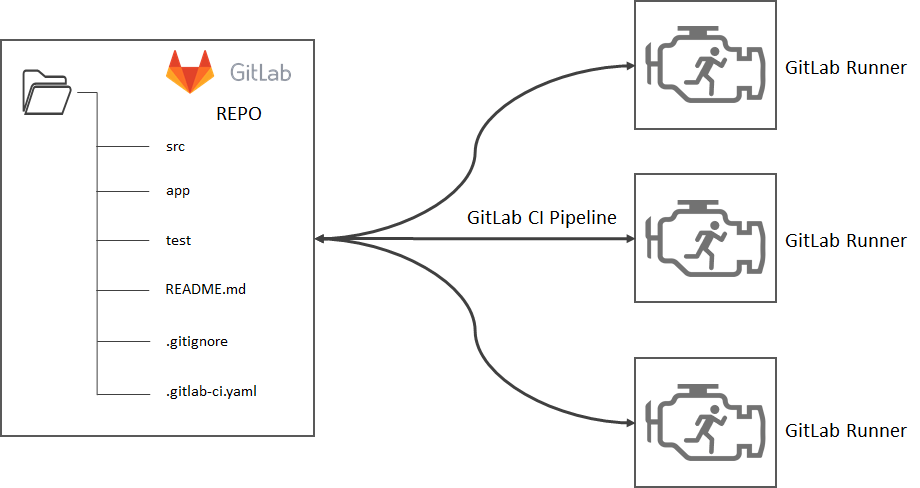
\includegraphics[width=14cm]{images/gitlab_runners.png}
	\caption{How GitLab Runners work (\cite{refGitLabRunners})}
	\label{fig:gitlab_runners}
\end{figure}

These Runners can also be self-hosted, meaning that not only is your codebase internal, but also the environments where your pipelines are run, increasing security and potentially reducing costs.
Configuring self-hosted Runners involves installing the Runner software on a suitable server, registering it with your GitLab instance, and then specifying that Runner in your 'gitlab-ci.yml' file.

\chapter{Infrastructure}

The infrastructure of the hosted GitLab service in our OpenStack platform consists of:
\begin{itemize}
    \item n Runners (at the moment 1) in a separate 'gitlabrunners' network, which is not public accessible
    \item One public facing server which hosts GitLab itself in the 'provider' network,
          the Runners need to access this server via the 'gitlabrunners' network
\end{itemize}

\section{Networks}

The 'gitlabrunners' network has a network address of '10.0.0.0/24' and a gateway IP of '10.0.0.254'.
The DHCP range is defined as '10.0.0.100-10.0.0.200'.\\

The Runners need to access the internet, for installation of packages/updates, but also for getting data to be used in the CI process (e.g. getting Docker images) 
That is the reason why also a router is added for this network.

\section{GitLab}

\subsection{Machine and network configuration}

A machine with flavor 'm1.large' with 'Debian-11' as base image is used for the machine of the self-hosted GitLab instance.
This is due to CPU, memory and software requirements of GitLab and Docker.\\

A floating IP is leased and used for the 'provider' network.
Due to the availability of the domain 'gruber.info', an A-record for the \ac{fqdn} 'gitlabtest.gruber.info' is used (\ref{fig:a_record}) and an https certificate is generated for that \ac{fqdn} via Let´s encrypt (\ref{fig:lets_encrypt}).
This certificate is used to prevent errors in the https communication.
\begin{figure}[H]
	\centering
	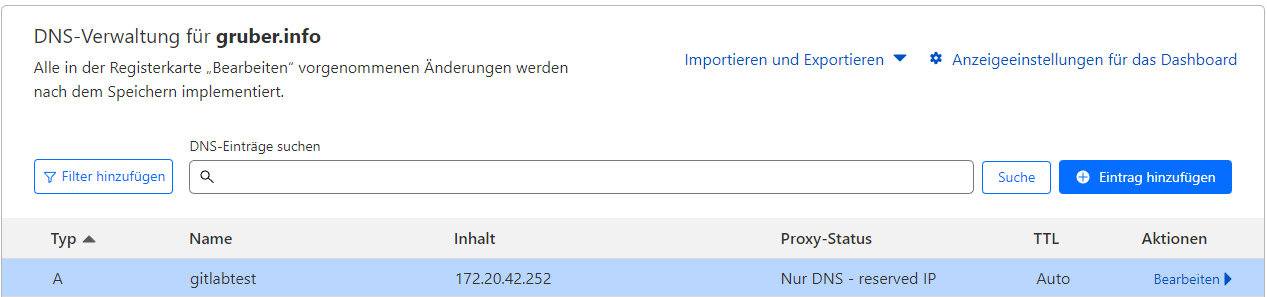
\includegraphics[width=14cm]{images/a-record.png}
	\caption{'gitlabtest.gruber.info' as A-record}
	\label{fig:a_record}
\end{figure}

\begin{figure}[H]
	\centering
	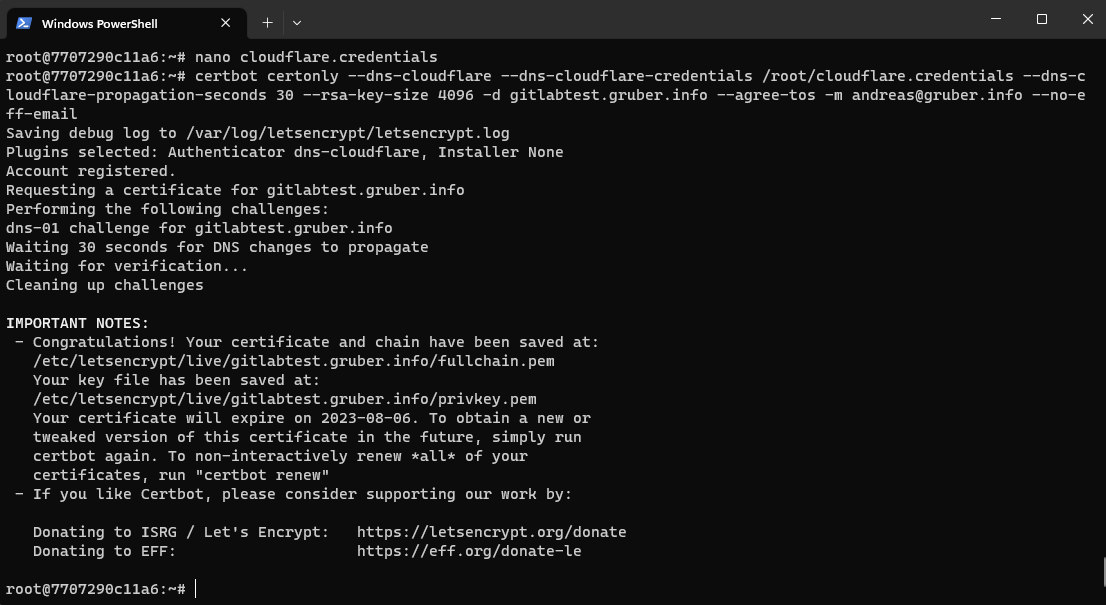
\includegraphics[width=14cm]{images/lets_encrypt.png}
	\caption{Let´s encrypt DNS-01 challenge}
	\label{fig:lets_encrypt}
\end{figure}

In the 'gitlabrunners' network a fixed IP of '10.0.0.99' is set for this machine, which can be used by the Runners to access GitLab.\\

\subsection{OS configuration}

Login to the OS is only possible via SSH and SSH keys. Login with password is not possible. 

As the 2GByte of memory is still not enough, a swap-file of 6GByte in size is added to the system (\ref{fig:swapfile}).
Without this, GitLab would not be able to start.

\begin{figure}[H]
	\centering
	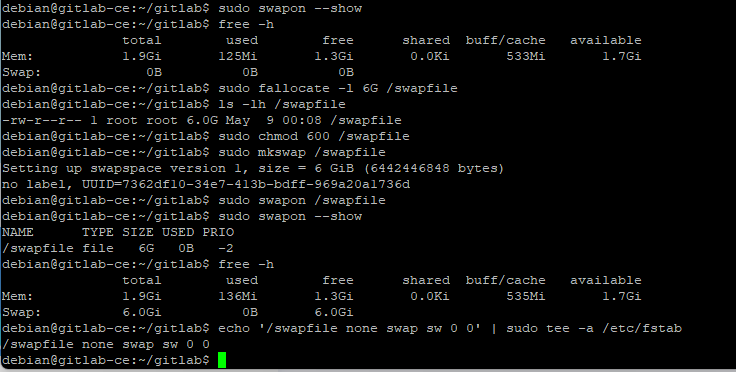
\includegraphics[width=14cm]{images/swapfile.png}
	\caption{Adding a swapfile}
	\label{fig:swapfile}
\end{figure}

Docker is installed according to the official Docker documentation (\cite{refDockerDebian}).

\chapter{Software}

\chapter{Verification and Testing}

\section{GitLab}

Make sure GitLab is accessible via https and the certificate is valid.
Just take a browser and go to 'https://gitlabtest.gruber.info' and verify the browser's response.

\begin{figure}[H]
	\centering
	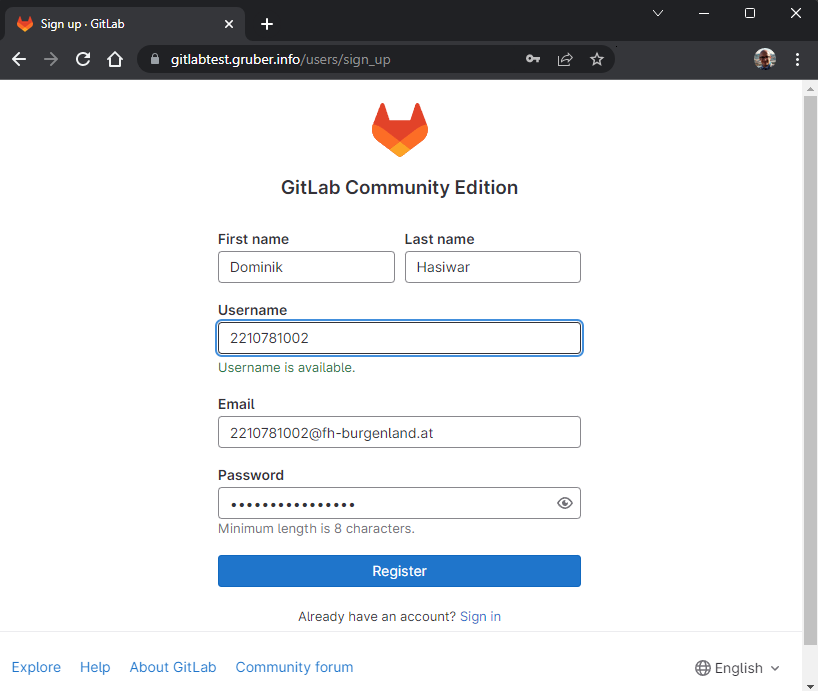
\includegraphics[width=14cm]{images/gitlab_signup.png}
	\caption{GitLab https response}
	\label{fig:gitlab_response}
\end{figure}
\  \\

The logs from GitLab can be accessed directly with the 'logs' command of 'docker compose':
\begin{lstlisting}[language=bash,caption={Manage GitLab},label={code:gitlab-logging}]
    # Open and follow to GitLab logs
    /home/debian/gitlab && docker compose logs -f
\end{lstlisting}

\section{GitLab Runners}

Verify if all added Runners are list in the Admin area of GitLab, see \ref{fig:gitlab_list_runners}.
If a Runner is not listed there, follow the 'Troubleshooting GitLab Runner' FAQ from GitLab (\cite{refGitLabRunnersTroubleshooting}).

\section{End-to-End test}

To verify all functionality all together, create a new project within GitLab, for example use the '.Net Core' template.
\begin{figure}[H]
	\centering
	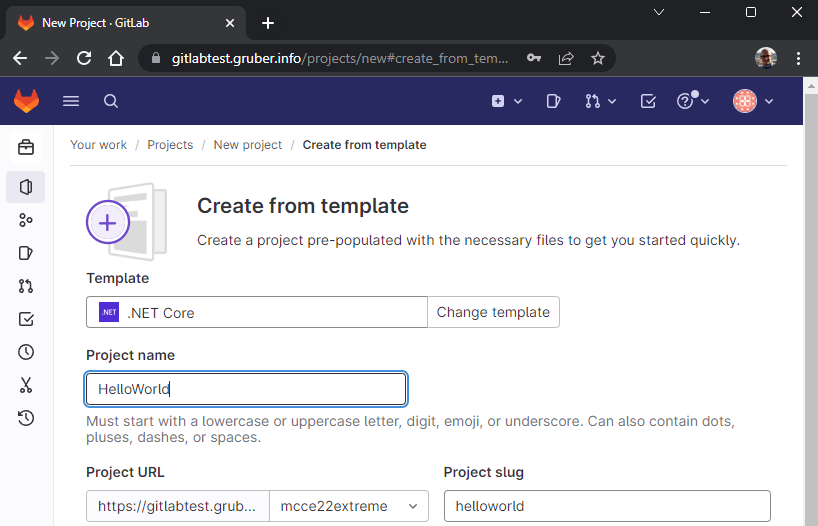
\includegraphics[width=14cm]{images/gitlab_create_project.png}
	\caption{GitLab create project}
	\label{fig:gitlab_create_project}
\end{figure}

Verify at the 'Jobs' list, if the jobs specified in the project are running successfully, see \ref{fig:gitlab_jobs_list}.
Failed jobs should be analyzed if the failure is in the infrastructure or in the code.
\begin{figure}[H]
	\centering
	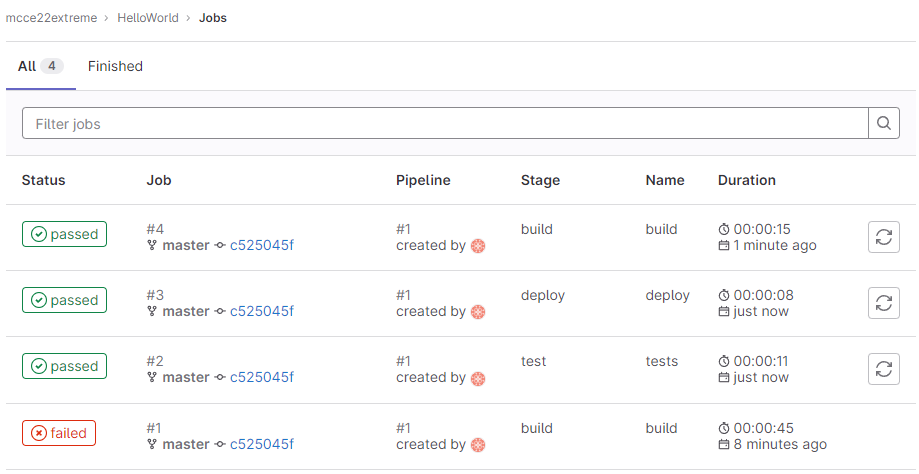
\includegraphics[width=14cm]{images/gitlab_jobs_list.png}
	\caption{List of jobs in GitLab project}
	\label{fig:gitlab_jobs_list}
\end{figure}
%	\begin{comment}

%\chapter{Verzeichnisse}
\cleardoublepage
%\appendix
%	\end{comment}
%\chapter{Verzeichnisse}
%http://stackoverflow.com/questions/1243342/how-to-avoid-a-page-break-before-start-of-bibliography
%\nocite{*}
\nocite{back2012web}
\begingroup
\let\clearpage\relax
\printbibliography[heading=bibnumbered] 
\endgroup

\noindent Das Literaturverzeichnis enthält alle Quellen (Bücher, Artikel, Internetquellen,..) in alphabetischer Reihenfolge in einem einzigen Verzeichnis, z.B.: 

\noindent Anmerkung: 

\noindent Es wird empfohlen, das Literaturverzeichnis von Beginn an mitzuführen und nicht die Quellenreferenzen in einem 2. Arbeitsgang einzusetzen

\newpage

%\bibliography{References}
\begingroup
\let\clearpage\relax
\listoffigures
\endgroup
\newpage

\begingroup
\let\clearpage\relax
\listoftables
\endgroup
\newpage
\chapter*{Formelverzeichnis}

Nur bei vielen Formeln und Abkürzungen erforderlich bzw. wenn von Betreuungsperson gewünscht.

\begingroup
\let\clearpage\relax
\vspace{-2.5cm}
\listofmyequations
\endgroup
\newpage


\chapter*{Abkürzungen}

\begin{acronym}
    \acro{aws}[AWS]{Amazon Web Services}
    \acro{cd}[CD]{Continuous Delivery/Continuous Deployment}
    \acro{ci}[CI]{Continuous Integration}
    \acro{fqdn}[FQDN]{Fully Qualified Domain Name}
    \acro{http}[HTTP]{Hypertext Transfer Protocol}
    \acro{https}[HTTPS]{Hypertext Transfer Protocol Secure}    
    \acro{iac}[IaC]{Infrastructure as Code}
    \acro{iot}[IoT]{Internet of Things}
    \acro{mqtt}[MQTT]{Message Queuing Telemetry Transport}
    \acro{s3}[S3]{Message Simple Storage Service}
    \acro{sca}[SCA]{Software Composition Analyse}
    \acro{sdlc}[SDLC]{Secure Development Lifecycle}
    \acro{saas}[SaaS]{Software as a Service}
    \acro{sast}[SAST]{Static Application Security Testing}  
    \acro{sdk}[SDK]{Software Development Kit}
    \acro{sns}[SNS]{Amazon Simple Notification Service}
    \acro{sqs}[SQS]{Amazon Simple Queue Service}
    \acro{wpf}[WPF]{Windows Presentation Foundation}    
\end{acronym}

\newpage
\addcontentsline{toc}{chapter}{Anhang}
\chapter*{Anhang}

Im Anhang sind all jene Informationen zu finden, die den Lesefluss der Arbeit stören würden, doch für die Vollständigkeit der Arbeit notwendig sind, z.B. Datentabellen, Fragebögen, etc.

\noindent Der Anhang unterliegt nicht mehr der Gliederung sondern wird mit Anhang A, Anhang B, … gekennzeichnet.

\end{document}
